\section{Methodology}\label{methodology}
    As this is a novel production method, there are a number of steps we must take in order to begin analyzing this process. We will make use of the ATLAS experiment's Athena software, which contains a number of helpful tools and wrappers around popular event generators, simulators, and reconstruction algorithms. There are three main steps for the production of the signal in the ATLAS experiment: testing and production of validation plots, approval from subgroup conveners, and submission of a ticket to generate events on the grid.

    \subsection{Testing and Production of Validation Plots}
        To start to generate events for our chosen process, we will use \textsc{MadGraph5\_aMC@NLO}, a popular program that is used for event generation and cross-section calculation. It comes equipped with many tools for doing these calculations within the regime of the standard model, but for anything outside of this, it requires a supplementary ``model'' that describes all of the details of the BSM process we want to simulate. The typical pipeline for this is to use the \textsc{FeynRules} package within Mathematica, from which a Universal FeynRules Output (UFO) model is produced that can be imported into \textsc{MadGraph5\_aMC@NLO}. Fortunately for us, models have already been made for the scalar LQ's; see Refs\cite{Dorsner_2018,Dorsner_2021}. A scenario with multiple LQ's present requires a simple combination of the individual models, and it is one such combination model that we will use.

        The Athena software in the ATLAS experiment provides the \mintinline{bash}{Gen_tf.py} ``transform'' script, which wraps around \textsc{MadGraph5\_aMC@NLO} and \textsc{Pythia8} (among other generators) and takes in a ``JobOptions'' file, a pseudo-Python script. The JobOptions file contains all the information relevant for event generation and parton showering. For instance, the desired process is specified using \textsc{MadGraph5\_aMC@NLO} syntax, Yukawa couplings, masses, and the number of events are specified, and filters can be added which apply generator-level kinemetic cuts. In the command line, the name of the output EVNT file is specified, which contains the raw event data after the showering is complete.

        The EVNT file cannot be directly parsed without considerable effort, so we need to produce so-called ``TRUTH derivations''. This is done with another one of Athena's transform scripts called \mintinline{bash}{Derivation_tf.py}, and requires only a few command-line inputs such as the input file and the name of the xAOD-formatted output file. There are a few different types of TRUTH formats which contain varying levels of the full truth record, from a direct copy of the EVNT data in xAOD format to a lite version that contains only the absolute necessary information for an analysis.

        Once the TRUTH derivations have been made, we can then apply a simple analysis using Athena's EventLoop framework, which is a tool that let's one easily parse through xAOD files and extract relevant information (among many others). Inside this analysis program, we can grab all of the kinematics for all of the final state particles, including the LQ's and their intermediate decay products. All that remains is to use ROOT to place them into histograms, which is a trivial exercise. Four example validation plots are shown in ~\ref{validationPlots}.
        
        \begin{figure}[ht]
            \centering
            
            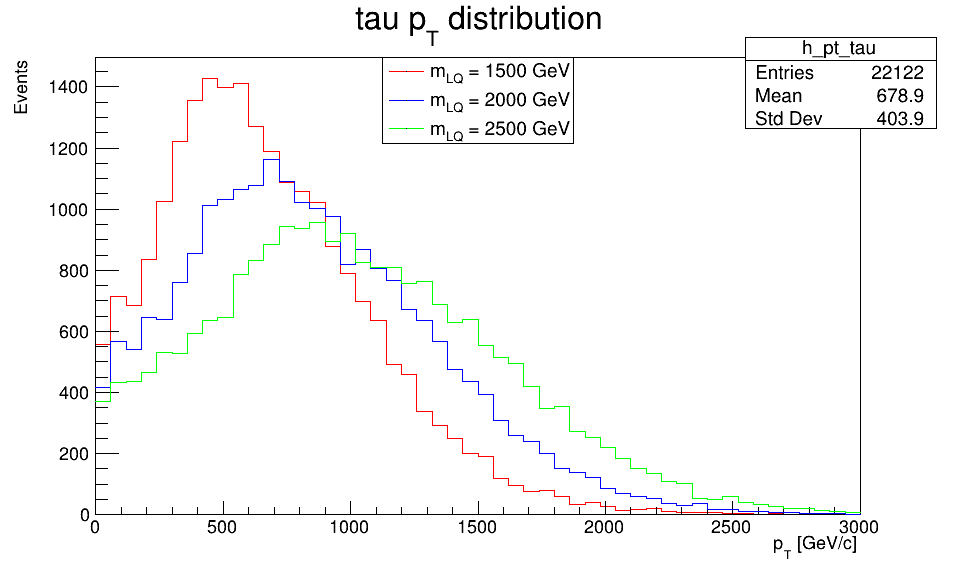
\includegraphics[scale=0.2]{res/ValidationPlots/h_pt_tau.png}
            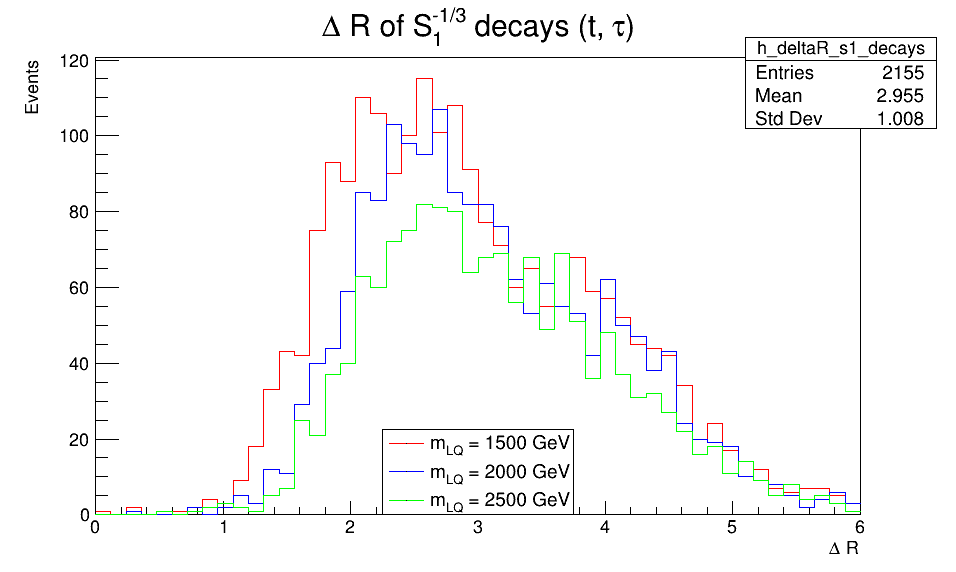
\includegraphics[scale=0.2]{res/ValidationPlots/h_deltaR_s1.png}
            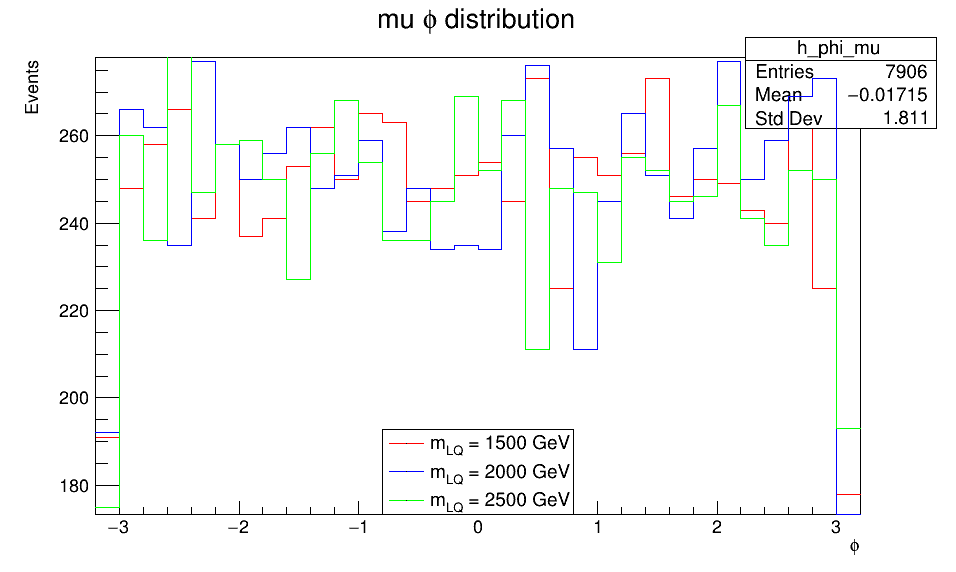
\includegraphics[scale=0.2]{res/ValidationPlots/h_phi_mu.png}
            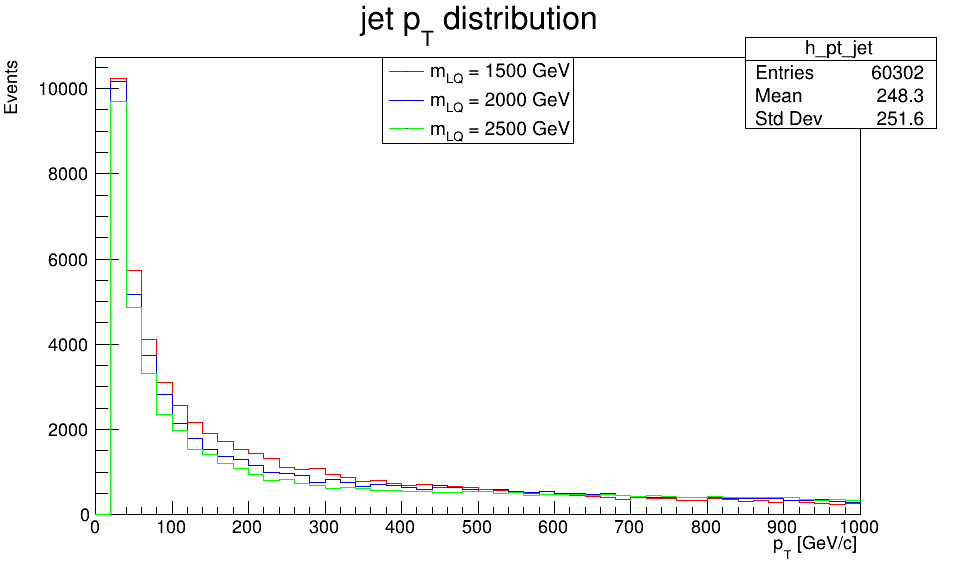
\includegraphics[scale=0.2]{res/ValidationPlots/h_pt_jet.png}

            \caption{Validation plots generated from test runs for the LQ model. Top left shows the $p_T$ distribution for the $\tau$ which came from the decay of the LQ's; top right shows the $\Delta R$ for the decay products ($t$ and $\tau$) of the $S_1$; bottom left shows the $\phi$ distribution for the final state $\mu$'s; and the bottom right shows the $p_T$ distribution for the produced jets.}
            \label{validationPlots}
        \end{figure}

    \subsection{Approval and Submission to the Grid}
        To make statistically valid predictions, we need to produce a very large number of events, more than could be reasonably produced even on a decently powerful single machine. Additionally, if the events are not produced within ATLAS (i.e. on a personal computer), their validity may be called into question. So, our events will need to be produced on ATLAS's central grid, which splits up the jobs and lets them all run in parallel on high-performance machines to improve efficiency. Before this can be done, approval must be granted by the relevent convening groups. In our case, this is the Lepton+X group, of which Tau+X is a subgroup. For documentation purposes, this was done here:~\url{https://indico.cern.ch/event/1439002/}. After approval is granted, we must submit a request with details about this approval, the relevant JobOptions files for each mass (or some other parameter) point, and a few additional details. Then, the ATLAS MC coordinators will run the generation, simulation, and reconstruction. This request was done here:~\url{https://its.cern.ch/jira/browse/ATLMCPROD-11359}

        
